\documentclass[a4paper,11.5pt,table]{article}
\usepackage[textwidth=170mm, textheight=230mm, inner=20mm, top=20mm, bottom=30mm]{geometry}
\usepackage[normalem]{ulem}
\usepackage[utf8]{inputenc}
\usepackage[T1]{fontenc}
\PassOptionsToPackage{defaults=hu-min}{magyar.ldf}
\usepackage[magyar]{babel}
\usepackage{amsmath, amsthm,amssymb, paralist, tikz, multirow}
\usetikzlibrary{arrows, positioning}

\usepackage{listings}
\lstset{
	language=C++, 
	basicstyle=\ttfamily, 
	keywordstyle=\color{blue}\ttfamily, 
	stringstyle=\color{red}\ttfamily,
	tabsize = 4
}

\usepackage{hyperref}

\begin{document}
	%%%%%%%%%%%RÖVIDÍTÉSEK%%%%%%%%%%
	\setlength\parindent{0pt}
	\def\<{<\hspace{0mm}<}
	
	\theoremstyle{definition}
	\newtheorem{note}{Megjegyzés}[subsection]
	%%%%%%%%%%%%%%%%%%%%%%%%%%%%%%%%%%%%%%%%%%%%%%%%%%%%%%%%%%%%%%%%%%%%%
	
	\begin{center}
		{\LARGE\textbf{C++}}
		
		{\Large Gyakorlat jegyzet}
		
		8. óra.
	\end{center}
	A jegyzetet \textsc{Umann} Kristóf készítette \textsc{Horváth} Gábor  előadásán. (\today)
	\section{Header fájlra és fordításra egységre szétbontás}
	Visszatérve a korábban írt láncolt listánkhoz, bátran állíthatjuk, hogy mindennel rendelkezik ami számunkra fontos. Azonban ha egy darab header fájlban tárolnánk mindent, számos problémába ütköznénk. Ha több fordítási egységbe illesztenénk be a headert, fordítási idejű hibát kapnánk, hogy számos függvényt többször próbáltunk definiálni (sértenénk az ODR-t). Erre megoldás lehet, hogy a definíciókat és deklarációkat elválasztjuk: az osztályban lévő függvények deklarációit hagyjuk meg a header fájlban, és a definíciókat egy külön fordítási egységbe tegyük!
	
	\begin{note}
		Feltűnhet majd, hogy pár definíció bent maradt. Erre később lesz magyarázat.
	\end{note}
	
	\medskip
	\fbox{\textbf{list.hpp:}}
\begin{lstlisting}
#ifndef LIST_H
#define LIST_H

#include <iosfwd>

class List;

class Iterator 
{
public:
	explicit Iterator(List *p) : p(p) {}
	bool operator==(Iterator other) const { return p == other.p; }
	bool operator!=(Iterator other) const { return !(*this == other); }
	Iterator operator++();
	int &operator*() const;
private:
	friend class ConstIterator;
	List *p;
};

class ConstIterator
{
public:
	ConstIterator(Iterator it) : p(it.p) {}
	explicit ConstIterator(const List *p) : p(p) {}
	bool operator==(ConstIterator other) const { return p == other.p; }
	bool operator!=(ConstIterator other) const { return !(*this == other); }
	ConstIterator operator++();
	int operator*() const;
private:
	const List *p;
};

class List 
{
public:
	explicit List(int data_, List *next = 0) : data(data_), next(next) {}
	~List() { delete next; }
	List(const List &other);
	List &operator=(const List &other);
	void add(int data);
	Iterator begin() { return Iterator(this); }
	ConstIterator begin() const { return ConstIterator(this); }
	Iterator end() { return Iterator(0); }
	ConstIterator end() const { return ConstIterator(0); }
private:
	friend Iterator;
	friend ConstIterator;
	int data;
	List *next;
};

#endif
\end{lstlisting}

	\fbox{\textbf{list.cpp:}}
\begin{lstlisting}
#include <iostream>

#include "list.hpp"
#include <iostream>

List::List(const List &other) : data(other.data), next(0) 
{
	if (other.next != 0) 
	{
		next = new List(*other.next);
	}
}

List& List::operator=(const List &other) 
{
	if (this == &other)
	return *this;
	delete next;
	data = other.data;
	if (other.next) 
	{
		next = new List(*other.next);
	} 
	else 
	{
		next = 0;
	}
	return *this;
}

void List::add(int data) 
{
	if (next == 0) 
	{
		next = new List(data);
	} 
	else 
	{
		next->add(data);
	}
}

Iterator Iterator::operator++() 
{
	p = p->next;
	return *this;
}

int& Iterator::operator*() const 
{
	return p->data;
}

ConstIterator ConstIterator::operator++() 
{
	p = p->next;
	return *this;
}

int ConstIterator::operator*() const 
{
	return p->data;
}
\end{lstlisting}
	\fbox{\textbf{main.cpp:}}
\begin{lstlisting}
#include <iostream>
#include "list.hpp"

void print(const List &l)
{
	for(ConstIterator it = l.begin(); it != begin(); ++it)
	{
		std::cout << *i << ' ';
	}
	std::cout << std::endl;
}

int main() {
	List head(5);
	head.add(8);
	head.add(10);
	head.add(8);
}

\end{lstlisting}
	
	Ez a szétválasztás sok egyéb előnnyel is jár: a \texttt{List}-hez tartozó információk sokkal kisebb helyen elférnek. Azonban ahogy a fenti megjegyzés is felhívta rá a figyelmet, a list.hpp továbbá is tartalmaz definíciókat! Ennek ellenére azt tapasztaljuk, hogyha több fordítási egységbe illesztjük be a headert, még akkor sem kapunk fordítási idejű hibát. Ennek a magyarázatához tegyünk egy kisebb kitérőt.
	\subsection{Inline függvények}
	
	Tekintsük azt a példát, amikor a \texttt{void f() \{\}} függvényt is beillesztjük a headerbe: több fordítási egység esetén linkelési hibát fog okozni, mert sértjük az ODR-t. Ez azonban megkerülhető az \texttt{inline} kulcsszó használatával, ez ugyanis megszünteti a linker hibát: minden inline-ként definiált függvény beilleszthető több fordítási egységbe, ahol linkelés folyamán a definíciók közül egy tetszőlegesen kiválasztásra kerül. Az osztályon belül kifejtett függvények implicit inline-ok, így sose okozhatnak fordítási hibát.
	
	\medskip
	A következő ábra jól demonstrálja a problémát:
	\begin{figure}[!h]
		\centering
		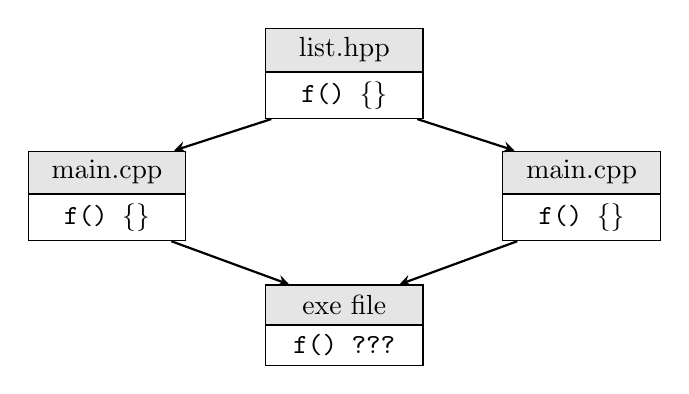
\begin{tikzpicture}
		\tikzstyle{HeaderName} = [rectangle, minimum width=2cm, minimum height=5mm, text centered, draw=black, fill= gray!20]
		\tikzstyle{CppName} = [rectangle, minimum width=2cm, minimum height=5mm, text centered, draw=black, fill= gray!20]
		\tikzstyle{FunctionName} = [rectangle, minimum width=2cm, minimum height=5mm, text centered, draw=black, fill= white]
		\tikzstyle{arrow} = [thick,->,>=stealth]
		
		
		\node (listHpp) [HeaderName] {list.hpp};
		\node (listHppF) [FunctionName, below = 0 mm of listHpp] {\texttt{f() \{\}}};
		
		\node (mainCpp) [CppName, below left = of listHpp] {main.cpp};
		\node (mainCppF) [FunctionName, below  = 0 mm of mainCpp] {\texttt{f() \{\}}};
		
		\node (listCpp) [CppName, below right = of listHpp] {main.cpp};
		\node (listCppF) [FunctionName, below  = 0 mm of listCpp] {\texttt{f() \{\}}};
		
		\node (exe) [CppName, below = 2.7 cm of listHpp] {exe file};
		\node (exeF) [FunctionName, below  = 0 mm of exe] {\texttt{f() ???}};
		
		\draw[arrow] (listHppF) -- (mainCpp);
		\draw[arrow] (listHppF) -- (listCpp);
		\draw[arrow] (mainCppF) -- (exe);
		\draw[arrow] (listCppF) -- (exe);
		\end{tikzpicture}
		\smallskip
		
		A \texttt{main.cpp}-ben vagy a \texttt{list.cpp}-ben lévő definíciója szerepeljen \texttt{f}-nek a futtatható fájlban?
	\end{figure}
	Az \texttt{f()} egy un. \textit{strong reference}-el jön létre ha nem inline, így a linker hibát dob ha több fordítási egységben definiálva van. Ha azonban inline-ként adjuk meg, akkor  \textit{weak reference}-ként értelmezi, a meglevő definíciók közül tetszőlegesen kerül egy kiválasztásra. Ez nyilván azt is jelenti, hogy minden ilyen függvény definíciójának meg kell egyeznie, hisz kellemetlen meglepetés érhet minket, ha különböző definíciók közül olyat választ a fordító, melyre nem számítanánk (és ez egyben nem definiált viselkedés is).
	\begin{note}
		A legtöbb fordítónál lehet egy LTO (\textit{link time optimalization}) funkciót bekapcsolni, mely a linkelésnél optimalizál, többek között ott végzi el az inlineolást.
	\end{note}
	\begin{note}
		Az inline függvények hajlamosak erősen megnövelni a bináris kódot, így az erőltetett használatuk nem javallott.
	\end{note}
	\begin{note}
		Az inline kulcsszó egy javaslat a fordítónak, de nem parancs. Nem inline függvények lehetnek inline-ok, és inlineként definiált függvények lehet mégsem lesznek azok.
	\end{note}
	Azok a tagfüggvények, melyek nem az osztály törzsében vannak definiálva, nem lesznek inline-ok, ezért volt az, hogy mielőtt szétszedtük a listánkat header fájlra és fordítási egységre, linkelési hibát kaptunk (\texttt{Iterator} és \texttt{ConstIterator} pár tagfüggvénye külön volt véve).
	\medskip
	
	Cseréljük le továbbá a print függvényt:
	
	\begin{lstlisting}
std::ostream& operator<<(std::ostream& os, const List &l)
{
	for(ConstIterator it = l.begin(); it != l.end(); ++it)
	{
		os << *it;
	}
	return os;
}
	\end{lstlisting}
	Sajnos fordítási hibát kapunk, hisz a fordító nem tudja mi az az \texttt{ostream}, így kell valamit include-olni. Ilyenkor a header fájlba inkább érdemes az \texttt{iosfwd} headert berakni \texttt{iostream} helyett, mert ez minden beolvasással és kiíratással kapcsolatos osztály/függvénynek csak a deklarációját tartalmazza, és így csökken a fordítási egység méretéte (azonban a cpp fájlban muszáj \texttt{iostream}-et használni, hogy a definíciók meglegyenek).
	\section{Névterek}
	
	A probléma csak az, hogy nagyon sok hasznos nevet elhasználtunk, pl. több \texttt{Iterator} nevű osztályt nem hozhatunk létre (az un. \textit{global namespace}-be kerültek), különben a névütközés áldozatai leszünk. Pedig várhatóan nem csak ennek az egy konténernek szeretnék iterátort írni. Megoldás lehet, hogyha az iterátorainkat egy névtérbe (\textit{namesspace}) rakjuk.
\begin{lstlisting}
namespace detail
{
	class Iterator
	{
		//...
	};
	class ConstIterator
	{
		//...
	};
}
\end{lstlisting}
	A névterek segíthetnek abba, hogy logikai egységebre rendezzük a programunkat. Az egyik legnagyobb ilyen egység az \texttt{std} névtér, mely tartalmaz minden függvényt, változót, stb, ami a standard részét alkotja. 
	
	Lehet névtereket egymásba is ágyazni, erre lehet példa a c++11-es \texttt{chrono} könyvtár, mely az \texttt{std} névteren belül számos dolgot a \texttt{chrono} alnévtérben tárol.
	
	\medskip
	Már csak az a baj, hogy így a \texttt{List} nem tudja, mi az az \texttt{Iterator}, hisz az egy \texttt{datail} nevű namespace-ben van, ezért vagy minden \texttt{Iterator}-t lecserélünk \texttt{detail::Iterator}-ra, vagy pedig létrehozunk egy szinonimát, melyet a \texttt{typedef} kulcsszóval tehetünk meg.
\begin{lstlisting}
class List
{
public:
	typedef detail::Iterator Iterator;
	typedef detail::ConstIterator ConstIterator;
	//...
};
\end{lstlisting}
	Ezzel a trükkel \texttt{List}-en belül (és csak ott!) elegendő lehet \texttt{Iterator}t írni. Ennek segítségével (mivel ezek a tpyedef-ek publikusak) így is lehet hivatkozni a \texttt{List} iterátorára: \texttt{List::Iterator}.
	
	\medskip
	Erre másik megoldás lehet, hogyha inline class-t hozunk létre, azaz az iterátor teljes deklarációját beillesztjük a \texttt{List}-be.
\begin{lstlisting}
class List
{
public:
	class Iterator
	{
		//...
	};
	//...
};
\end{lstlisting}
	\section{Nem template osztály átírása template osztályra}
	Már csak az a probléma, hogy ez az osztály csak \texttt{int}-ekre működik. Csináljunk belőle inkább egy template osztályt! Feladatunk csupán annyi, hogy az osztály elé írjunk egy \texttt{template <typename T>}-t, és minden \texttt{List}-et \texttt{List<T>}-re cseréljünk, és minden \texttt{int}-et \texttt{T}-re. Ehhez nyilván az iterátorainkat is módosítani kell.
	
	\medskip
	Időközben felmerül a hatékonyság kérdése is. A listánkban eddig mindent érték szerint vettünk át, ami \texttt{int}-nél (általában) hatékonyabb, mint a referencia szerinti, azonban template-eknél nem garantáljuk, hogy ilyen alap típussal fogják példányosítani az osztályunkat, és ilyenkor úgy szokás hozzáállni, hogy a leendő template paraméter egy nagyon nagy mérettel rendelkező típus lesz, melynél érték helyett konstans referenciával szokás átvenni minden paramétert hatékonyság végett. Sőt, még a \texttt{ConstIterator} dereferáló operátora is inkább konstans referenciát adjon vissza!
	\begin{note}
		Általában egy primitív típus, mint pl. az \texttt{int} vagy \texttt{char}, kisebb mérettel rendelkezik mint a hozzá tartozó pointer vagy referencia típus, így hatákonyabb ezeket a típusokat inkább érték szerint átvenni.
	\end{note}
	
	\fbox{\textbf{list.hpp:}}
\begin{lstlisting}
#ifndef LIST_H
#define LIST_H

#include <iosfwd>

template<typename T>
class List;

namespace detail 
{
	template<typename T>
	class Iterator
	{
	public:
		explicit Iterator(List<T> *p) : p(p) {}
		bool operator==(Iterator other) const { return p == other.p; }
		bool operator!=(Iterator other) const { return !(*this == other); }
		Iterator operator++();
		T &operator*() const;
	private:
		template<typename>
		friend class ConstIterator;
		List<T> *p;
	};
	
	template<typename T>
	class ConstIterator
	{
	public:
		ConstIterator(Iterator<T> it) : p(it.p) {}
		explicit ConstIterator(const List<T> *p) : p(p) {}
		bool operator==(ConstIterator other) const { return p == other.p; }
		bool operator!=(ConstIterator other) const { return !(*this == other); }
		ConstIterator operator++();
		const T &operator*() const;
	private:
		const List<T> *p;
	};	
}

template <typename T>
class List 
{
public:
	typedef detail::Iterator<T> Iterator;
	typedef detail::ConstIterator<T> ConstIterator;
	explicit List(const T &data_, List *next = 0) : data(data_), next(next) {}
	~List() { delete next; }
	List(const List &other);
	List &operator=(const List &other);
	void add(const T &data);
	Iterator begin() { return Iterator(this); }
	ConstIterator begin() const { return ConstIterator(this); }
	Iterator end() { return Iterator(0); }
	ConstIterator end() const { return ConstIterator(0); }
private:
	friend Iterator;
	friend ConstIterator;
	T data;
	List *next;
};

template<typename T>
std::ostream &operator<<(std::ostream& os, const List<T> &l);

#endif
\end{lstlisting}
	\fbox{\textbf{list.cpp:}}
\begin{lstlisting}
#include "list.hpp"
#include <iostream>

template<typename T>
List<T>::List(const List &other) : data(other.data), next(0) 
{
	if (other.next != 0) 
	{
		next = new List(*other.next);
	}
}

template<typename T>
List<T> &List<T>::operator=(const List<T> &other) 
{
	if (this == &other)
	return *this;
	delete next;
	data = other.data;
	if (other.next) 
	{
		next = new List(*other.next);
	} 
	else 
	{
		next = 0;
	}
	return *this;
}

template <typename T>
void List<T>::add(const T &data) 
{
	if (next == 0) 
	{
		next = new List(data);
	} 
	else 
	{
		next->add(data);
	}
}

namespace detail 
{
	template <typename T>
	Iterator<T> Iterator<T>::operator++() 
	{
		p = p->next;
		return *this;
	}
	
	template <typename T>
	T &Iterator<T>::operator*() const 
	{
		return p->data;
	}
	
	template <typename T>
	ConstIterator<T> ConstIterator<T>::operator++() 
	{
		p = p->next;
		return *this;
	}
	
	template <typename T>
	const T &ConstIterator<T>::operator*() const 
	{
		return p->data;
	}
}

template<typename T>
std::ostream &operator<<(std::ostream& os, const List<T> &l) 
{
	for(List<T>::ConstIterator it = l.begin(); it != l.end(); ++it) 
	{
		os << *it << ' ';
	}
	os << std::endl;
	return os;
}
\end{lstlisting}
	Itt a kiírató operátorunk miatt nem fog fordulni a kódunk! A \texttt{ConstIterator} {dependent scope}-ban lesz (ld. 7. gyakorlat).
	
	\begin{lstlisting}
template<typename T>
std::ostream &operator<<(std::ostream& os, const List<T> &l) 
{
	for(typename List<T>::ConstIterator it = l.begin(); it != l.end(); ++it) 
	{
		os << *it << ' ';
	}
	os << std::endl;
	return os;
}
	\end{lstlisting}
	
	\fbox{\textbf{main.cpp}}
	\begin{lstlisting}
#include <iostream>
#include "list.hpp"

int main() 
{
	List<int> head(5); // *
	head.add(8);
	head.add(10);
	head.add(8);
	std::cout << head;
}
	\end{lstlisting}
	
	Kérdés, hogy a megjelölt helyen kell-e typename vagy sem? A válasz az hogy nem, mert itt az \texttt{int} egy ismert típus, az előbbi példában meg \texttt{T} nem volt ismert, és az aztán bármi lehetett. A fordító a konkrét behelyettesítésnél tudni fogja, hogy \texttt{ConstIterator} egy típus lesz.
	
	\medskip
	No, fordítsunk!
	
	\medskip
	Igen, sejthető volt hogy ez nem fog menni. Úgy tűnhet, hogy semmi se úgy működik ebbe a nyelvbe, ahogy azt gondolnánk. Mindenre van magyarázat,
	\begin{center}
		\textit{,,néha az hogy valaki elkúrta.''}
		
		/Horváth Gábor/
	\end{center}
	Linkelési hibát kaptunk, de miért? A list.hpp-ben benne van mindenféle deklaráció, és a list.cpp-ben meg több \texttt{List}-béli implementáció. Amikor a list.cpp-t fordítjuk, létrejön az object fájl, a mainben szintén. Azonban minden implementált függvény template: a háttérben a list.cpp-ben semmit sem példányosítunk, így az szinte teljesen üres fordítás után. A main.cpp-ben így hiába megy az object fájl kreálása, lévén nem kell ismerni ahhoz a függvények definícióit, azonban a linkelésnél már meg kéne tudnunk találni azokat. Így a template osztályokat/függvényeket a header fájlokban kell tárolni.
	
	Itt megoldás lehet, hogyha az egész cpp-t beemeljük a list.hpp-be (itt mát azonban muszáj lesz az \texttt{iosfwd}-t \texttt{iostream}-re váltani). Az átláthatóság azonban nem lett áldozat, mert a fájl tetején van a deklaráció, és szétszedve van benne definíció.
	
\end{document}
